\documentclass[class=report, crop=false, 12pt,a4paper]{standalone}
\usepackage{enumitem}
\usepackage{multicol}
\usepackage{graphicx}
\usepackage{float}
\usepackage{amsmath}
\usepackage{amssymb}
\usepackage{mathtools}
\usepackage{siunitx}
\usepackage{commath}
\usepackage{array}
\usepackage{natbib}
\usepackage{tikz}
\usepackage{cancel}
\usepackage[a4paper,width=150mm,top=25mm,bottom=25mm]{geometry}
\allowdisplaybreaks
\setlength{\parindent}{0pt}
\numberwithin{equation}{section}
\begin{document}
\begin{center}
  02/03/2021
\end{center}
\section{Overview of a Steam Power Plant}
\subsection{Schematic of A Steam Power System}
\begin{figure}[H]
  \centering
  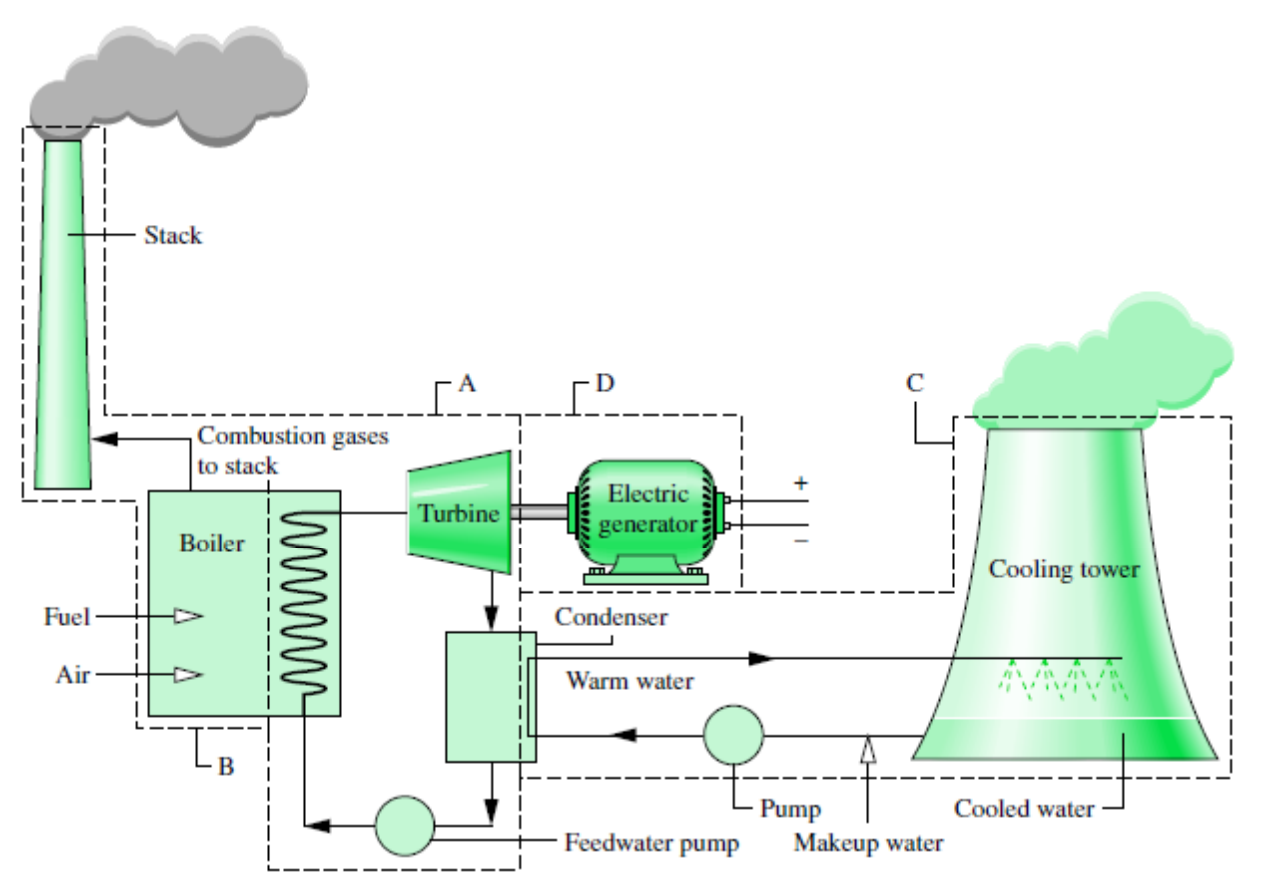
\includegraphics[width = 1 \textwidth]{../img/diagram136.png}
  \caption{}
\end{figure}
\subsection{Pressurised-water Reactor Nuclear Steam Power Plant}
\begin{figure}[H]
  \centering
  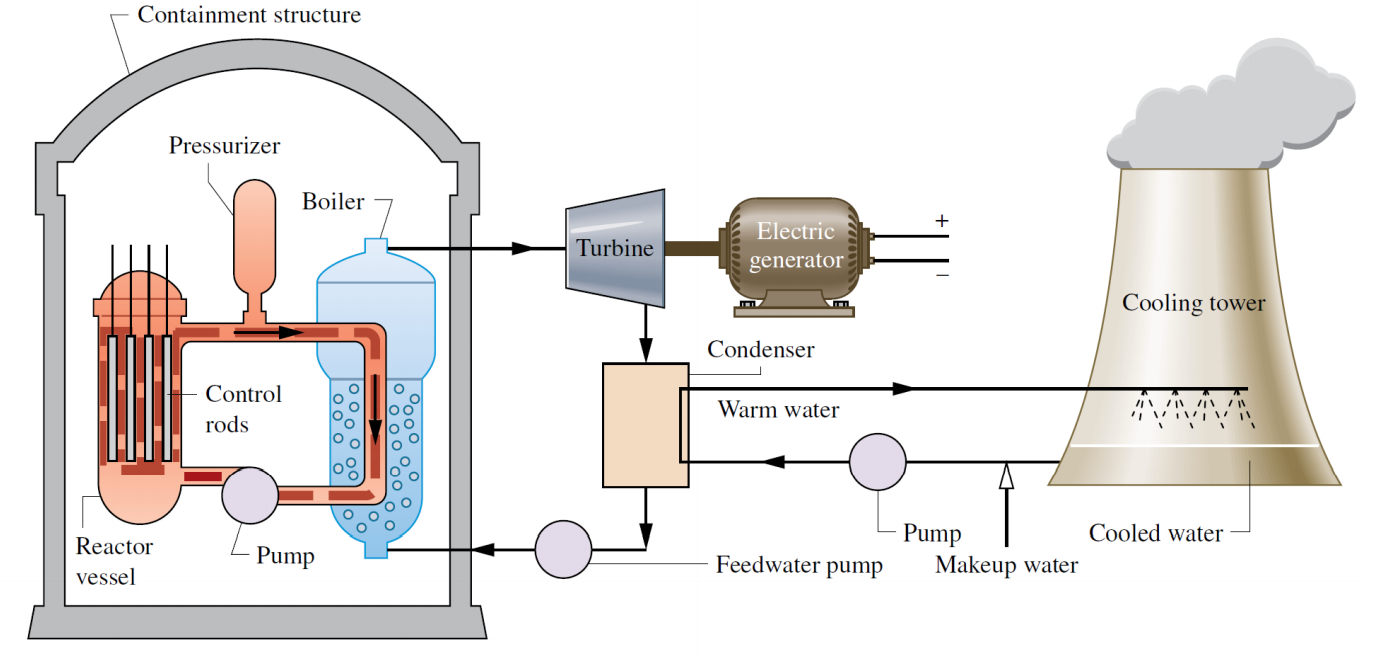
\includegraphics[width = 1 \textwidth]{../img/diagram137.png}
  \caption{}
\end{figure}
\subsection{Concentrating Solar Thermal Steam Power Plant}
\begin{figure}[H]
  \centering
  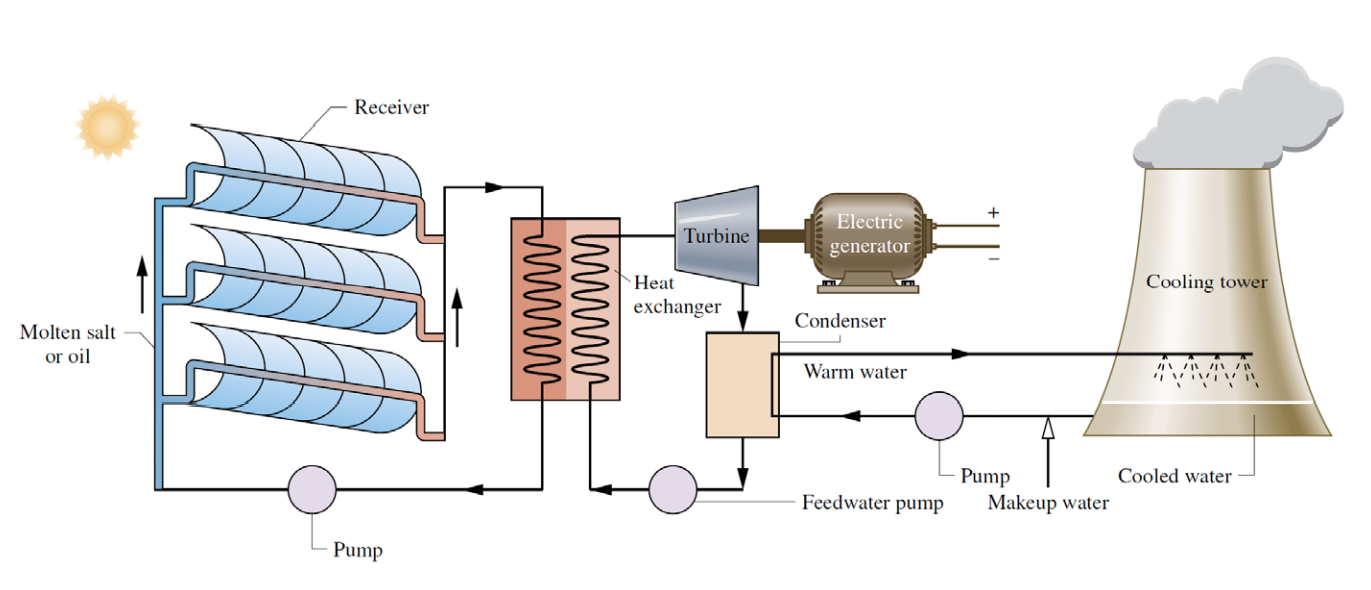
\includegraphics[width = 1 \textwidth]{../img/diagram138.png}
  \caption{}
\end{figure}
\subsection{Geothermal Vapour Power Plant}
\begin{figure}[H]
  \centering
  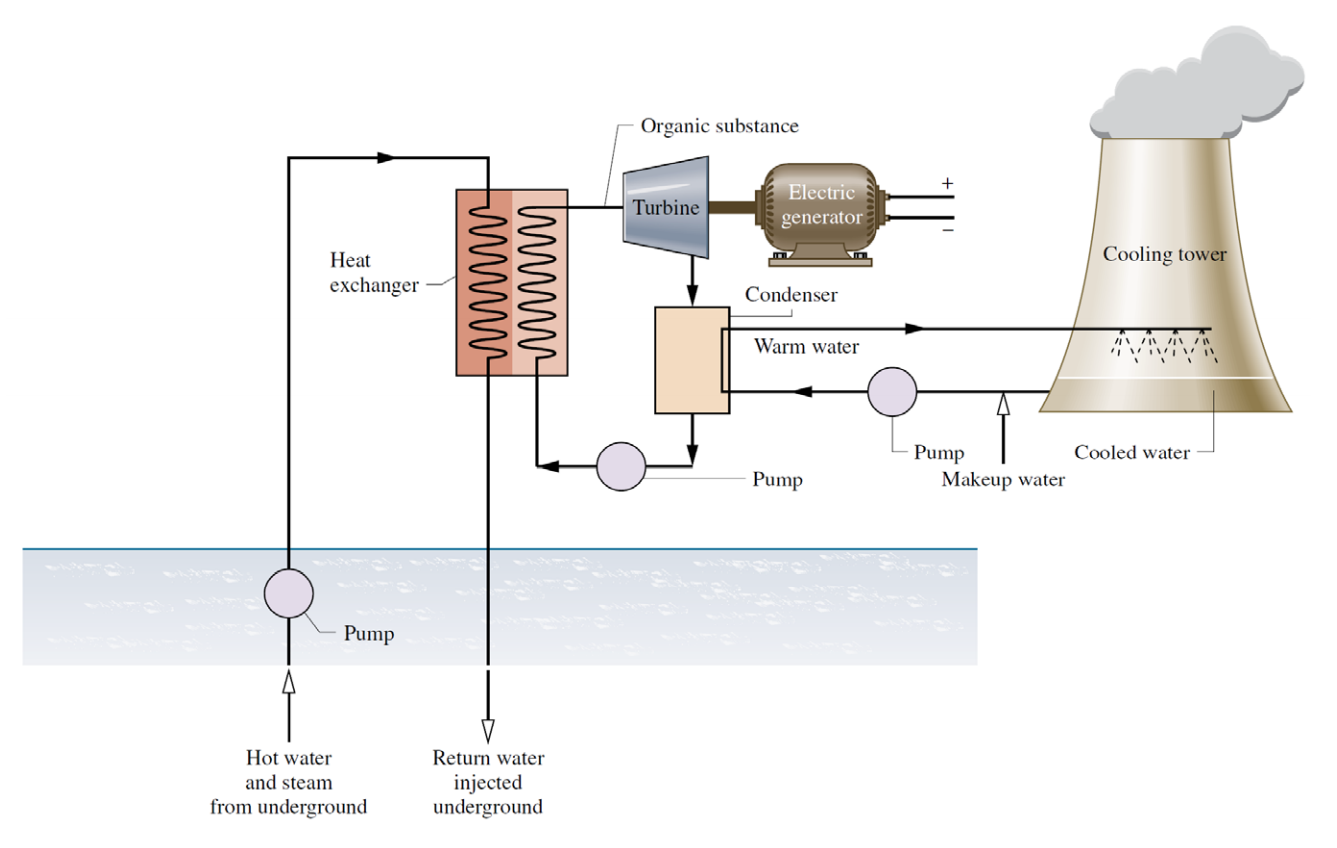
\includegraphics[width = 1 \textwidth]{../img/diagram139.png}
  \caption{}
\end{figure}
\subsection{Main Components of a Steam Power System}
\begin{figure}[H]
  \centering
  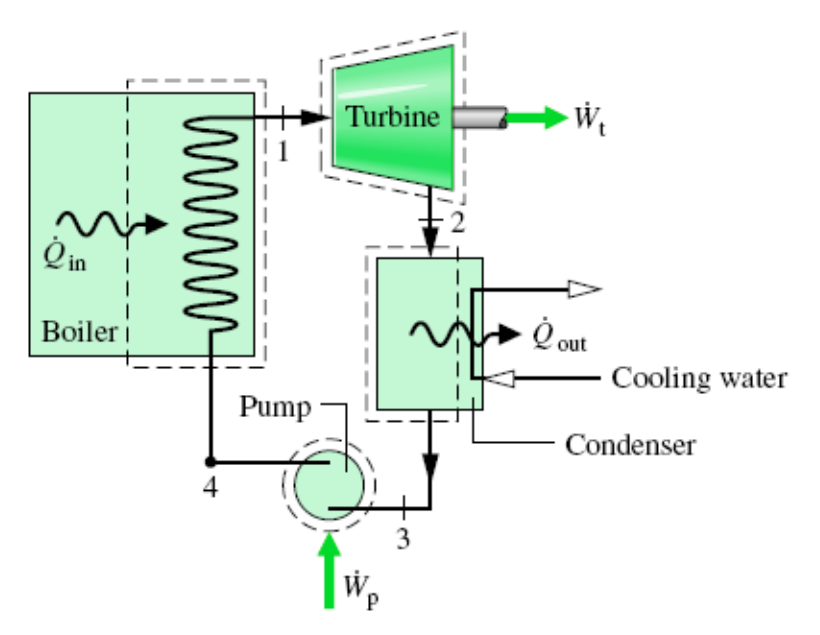
\includegraphics[width = 0.65 \textwidth]{../img/diagram140.png}
  \caption{}
\end{figure}
\begin{itemize}[noitemsep]
  \item Turbine
  \item Condenser
  \item Pump
  \item Boiler (Steam Generator)
\end{itemize}
\subsection{Work and Heat Transfer}
\subsubsection{Turbine:}
\begin{gather}
  0 = \cancel{\dot{Q}_{CV}} - \dot{W}_t + \dot{m}\left[h_1 - h_2 + \cancel{\frac{V_1^2-V_2^2}{2}} + \cancel{g(z_1-z_2)}\right] \\[5pt]
  \frac{\dot{W}_t}{\dot{m}} = h_1 - h_2
\end{gather}
\subsubsection{Conderser:}
\begin{gather}
  \frac{\dot{Q}_{out}}{\dot{m}} = h_2-h_3
\end{gather}
\subsubsection{Pump:}
\begin{gather}
  \frac{\dot{W}_p}{\dot{m}} = h_4-h_3
\end{gather}
\subsubsection{Boiler:}
\begin{gather}
  \frac{\dot{Q}_{in}}{\dot{m}} = h_1-h_4
\end{gather}
\section{The Carnot Vapour Power Cycle}
\begin{figure}[H]
  \centering
  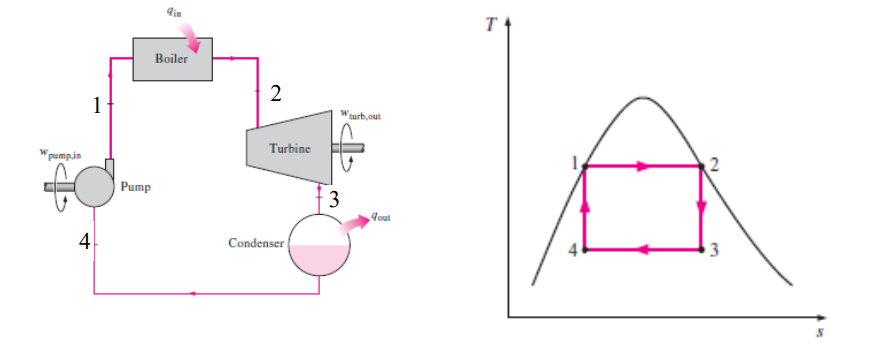
\includegraphics[width = 1 \textwidth]{../img/diagram141.png}
  \caption{}
\end{figure}
\begin{itemize}[noitemsep]
  \item \textbf{Process $\mathbf{1\rightarrow 2}$}: The working fluid is heated reversibly and isothermally in a boiler
  \item \textbf{Process $\mathbf{2\rightarrow 3}$}: then expanded isentropically in a turbine
  \item \textbf{Process $\mathbf{3\rightarrow 4}$}: subsequently condensed reversibly and isothermally in a condenser
  \item \textbf{Process $\mathbf{4\rightarrow 1}$}: and finally compressed isentropically by a compressor to the initial state
\end{itemize}
\subsection{Problems with the Carnot Vapour Power Cycle}
The quality of the steam decreases during \textbf{isentropic expansion process (process 2-3)}, leading to steam with a high moisture content. The impingement of \textbf{liquid droplets} on the turbine blades causes \textbf{erosion} and is a major source of wear. Usually, steam with quality less than about \textbf{90 percent} cannot be tolerated in the operation of power plants. \\\\
The \textbf{isentropic compression process (process 4-1)} involves the compression of a liquid–vapor mixture to a saturated liquid. Problems:
\begin{itemize}[noitemsep]
  \item It is \textbf{not easy to control the condensation process} so precisely as to end up with the desired quality at state 4.
  \item It is \textbf{not practical to design a compressor that handles two phases}.
\end{itemize}
Thus, the idealised Carnot Vapour Cycle is not practical!
\section{Rankine Vapour Power Cycle}
\begin{figure}[H]
  \centering
  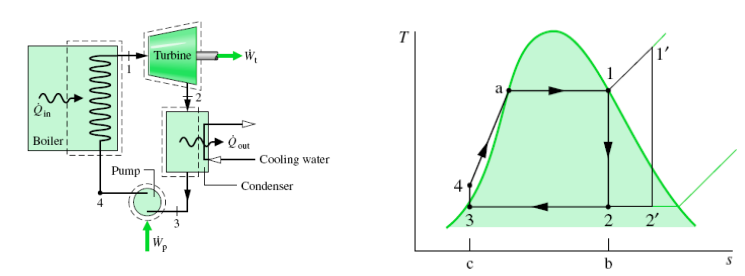
\includegraphics[width = 1 \textwidth]{../img/diagram142.png}
  \caption{}
\end{figure}
\begin{itemize}[noitemsep]
  \item \textbf{Process $\mathbf{1\rightarrow 2 \ \text{or} \ (1'\rightarrow 2')}$}: Isentropic expansion of the working fluid \textbf{(Saturated or Superheated Vapor)} through the turbine to the condenser pressure.
  \item \textbf{Process $\mathbf{2\rightarrow 3 \ (2'\rightarrow 3')}$}: Heat transfer from the working fluid as it flows at constant pressure through the condenser with \textbf{saturated liquid at state 3}.
  \item \textbf{Process $\mathbf{3\rightarrow 4}$}: Isentropic compression in the pump to state 4 in the compressed liquid region.
  \item \textbf{Process $\mathbf{4\rightarrow 1 \ (4'\rightarrow 1')}$}: Heat transfer to the working fluid as it flows at constant pressure through the boiler to complete the cycle.
\end{itemize}
Area 1–b–c–4–a–1 represents the heat transfer to the working fluid passing through the boiler:
\begin{gather}
  q_{in}=(h_1-h_4)
\end{gather}
Area 2–b–c–3–2, is the heat transfer from the working fluid passing through the condenser, each per unit of mass flowing: 
\begin{gather}
  q_{out}=(h_2-h_3)
\end{gather}
The enclosed area 1–2–3–4–a–1 can be interpreted as the net heat input or, equivalently, the net work output, per unit mass of the working fluid:
\begin{gather}
  w_{net}=(h_1-h_4)-(h_2-h_3)
\end{gather}
\subsection{Key Parameters of Ideal Rankine Cycle:}
\subsubsection{Thermal Efficiency:}
\begin{gather}
  \eta = \frac{\frac{\dot{W}_t}{\dot{m}} - \frac{\dot{W}_p}{\dot{m}}}{\frac{\dot{Q}_{in}}{\dot{m}}} = \frac{(h_1-h_2)-(h_4-h_3)}{h_1-h_4} \\[5pt]
  \eta = \frac{\frac{\dot{Q}_{in}}{\dot{m}} - \frac{\dot{Q}_{out}}{\dot{m}}}{\frac{\dot{Q}_{in}}{\dot{m}}} = 1-\frac{\frac{\dot{Q}_{out}}{\dot{m}}}{\frac{\dot{Q}_{in}}{\dot{m}}} \\[5pt]
  = 1-\frac{(h_2-h_3)}{(h_1-h_4)} \\[5pt]
  \text{Neglect Pump Power:} \\[5pt]
  \eta = \frac{h_1-h_2}{h_1-h_3}
\end{gather}
\subsubsection{The Back Work Ratio:}
\begin{gather}
  \text{bwr} = \frac{\frac{\dot{W}_p}{\dot{m}}}{\frac{\dot{W}_t}{\dot{m}}} = \frac{(h_4-h_3)}{(h_1-h_2)}
\end{gather}
\subsubsection{Pump Power:}
\begin{gather}
  \left(\frac{\dot{W}_p}{\dot{m}}\right)\mathop{_{int}}_{rev} = \int_{3}^{4}v \ dp \\[5pt]
  \longrightarrow \text{Incompressible Assumption:} \\[5pt]
  \left(\frac{\dot{W}_p}{\dot{m}}\right)\mathop{_{int}}_{rev} \approx v_3(p_4-p_3)
\end{gather}
\subsection{The Effect of Temperature on Thermal Efficiency}
Heat input (internally reversible process):
\begin{gather}
  \left(\frac{\dot{Q}_{in}}{\dot{m}}\right)\mathop{_{int}}_{rev} = \int_{4}^{1}T \ ds = \text{area 1-b-c-4-a-1}
\end{gather}
Average high temperature:
\begin{gather}
  \left(\frac{\dot{Q}_{in}}{\dot{m}}\right)\mathop{_{int}}_{rev} = \overline{T}_{in}(s_1-s_4)
\end{gather}
Heat output (internally reversible process):
\begin{gather}
  \left(\frac{\dot{Q}_{out}}{\dot{m}}\right)\mathop{_{int}}_{rev} = T_{out}(s_2-s_3) = \text{area 2-b-c-3-2}
\end{gather}
Low temperature:
\begin{gather}
  \left(\frac{\dot{Q}_{out}}{\dot{m}}\right)\mathop{_{int}}_{rev} = T_{out}(s_1-s_4)
\end{gather}
For internally reversible cycle: 
\begin{gather}
  \eta_{ideal} = 1-\frac{\left(\frac{\dot{Q}_{out}}{\dot{m}}\right)\mathop{_{int}}_{rev}}{\left(\frac{\dot{Q}_{in}}{\dot{m}}\right)\mathop{_{int}}_{rev}} = 1-\frac{T_{out}}{\overline{T}_{in}}
\end{gather}
\subsection{Increasing the Efficiency of the Rankine Cycle}
\subsection*{Lowering the Condenser Pressure (Lowering the Low temperature):}
\begin{figure}[H]
  \centering
  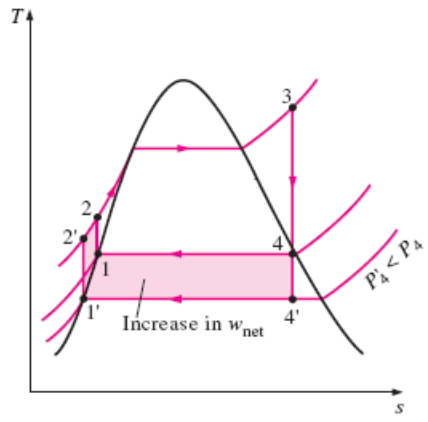
\includegraphics[width = 0.45 \textwidth]{../img/diagram143.png}
  \caption{}
\end{figure}
The colored area on this diagram represents the increase in net work output as a result of lowering the condenser pressure. \\\\
The heat input requirements also increase but this increase is very small. \\\\
\textbf{The overall effect of lowering the condenser pressure is an increase} in the thermal efficiency of the cycle. \\\\
\textbf{The condenser pressure cannot be lower than the saturation pressure corresponding to the ambient temperature}.
\subsection*{Superheating the Steam to Higher Temperatures:}
\begin{figure}[H]
  \centering
  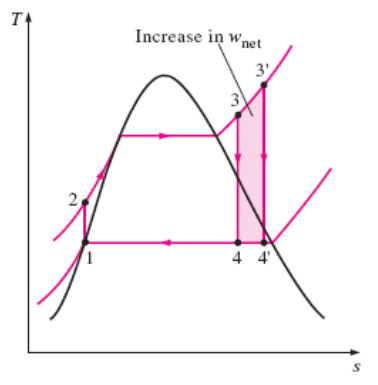
\includegraphics[width = 0.45 \textwidth]{../img/diagram144.png}
  \caption{}
\end{figure}
Both the net work and heat input increase, however, the overall effect is an increase in thermal efficiency since the \textbf{average high temperature} increases. \\\\
Another desirable effect: It decreases the moisture content of the steam at the turbine exit. \\\\
The temperature to which steam can be superheated is limited by metallurgical considerations:
\begin{itemize}[noitemsep]
  \item Presently the highest steam temperature allowed at the turbine inlet is about $\mathbf{620\si{\si\degree}C}$
  \item Any increase in this value depends on improving the materials used or finding new ones that can withstand higher temperatures
  \item \textbf{Ceramics} are very promising in this regard
\end{itemize}
\subsection*{Increasing the Boiler Pressure:}
\begin{figure}[H]
  \centering
  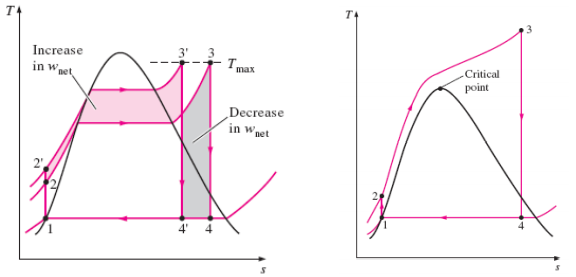
\includegraphics[width = 0.85 \textwidth]{../img/diagram145.png}
  \caption{A supercritical Rankine cycle}
\end{figure}
Raises the average temperature at which heat is transferred to the steam and thus raises the thermal efficiency of the cycle. \\\\
Notice that for a fixed turbine inlet temperature, the cycle shifts to the left and \textbf{the moisture content of steam at the turbine exit increases}. This undesirable side effect can be corrected, however, by reheating the steam, as discussed in the next section. \\\\
Today advanced modern steam power plants operate at \textbf{supercritical pressures (up to 30 MPa)} and have thermal efficiencies of up to \textbf{47 percent} for fossil fuel plants and \textbf{35 percent} for nuclear plants.
\subsection{The Ideal Reheat Rankine Cycle}
Superheat the steam to very high temperatures before it enters the turbine. 
Expand the steam in the turbine in two stages, and reheat it in between. 
\begin{figure}[H]
  \centering
  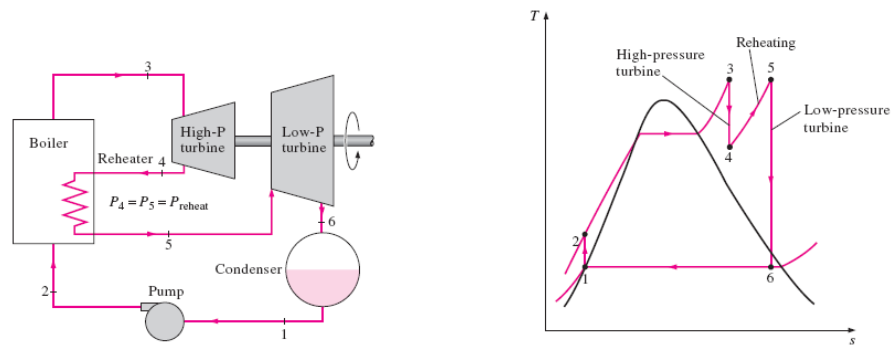
\includegraphics[width = 1 \textwidth]{../img/diagram146.png}
  \caption{}
\end{figure}
Total heat input:
\begin{gather}
  q_{in} = q_{primary} + q_{reheat} = (h_3-h_2) + (h_5-h_4)
\end{gather}
Total turbine work output:
\begin{gather}
  w_{turb,out} = w_{turb,I} + w_{turb,II} = (h_3-h_4) + (h_5-h_6)
\end{gather}
The incorporation of a single reheat stage in a modern power plant improves the cycle efficiency by 4 to 5 percent. The average temperature during the reheat process can be increased by increasing the number of expansion and reheat stages:
\begin{itemize}[noitemsep]
  \item The effect of performance improvement decreases with the increasing number of the reheat
  \item Normally, 1-2 stages of reheat are used in practice.
\end{itemize}
\begin{figure}[H]
  \centering
  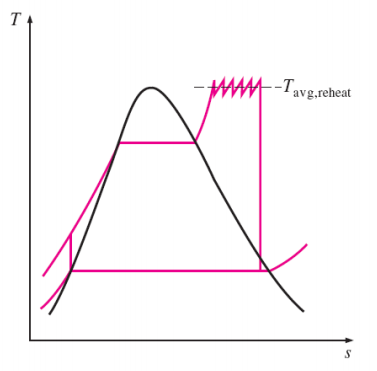
\includegraphics[width = 0.45 \textwidth]{../img/diagram147.png}
  \caption{}
\end{figure}
\subsection{Principal Irreversibilities and Losses}
\begin{figure}[H]
  \centering
  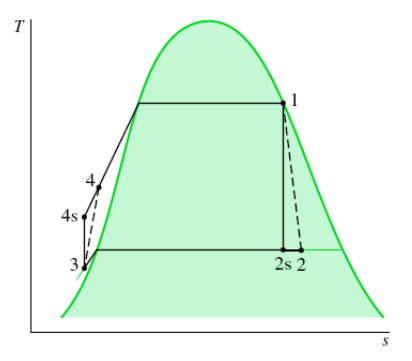
\includegraphics[width = 0.45 \textwidth]{../img/diagram148.png}
  \caption{}
\end{figure}
\subsubsection{Turbine:}
Heat transfer from the turbine to the surroundings represents a loss, but since it is usually of secondary importance, it often can be neglected. \\\\
The principal irreversibility experienced by the working fluid is associated with the expansion through the turbine. The isentropic turbine efficiency allows the effect of irreversibilities within the turbine to be accounted for in terms of the actual and isentropic work amounts:
\begin{gather}
  \eta_t = \frac{\left(\frac{\dot{W}_t}{\dot{m}}\right)}{\left(\frac{\dot{W}_t}{\dot{m}}\right)_s} = \frac{h_1-h_2}{h_1-h_{2s}}
\end{gather}
\subsubsection{Pump:}
The work input to the pump required to overcome frictional effects also reduces the net power output of the plant. The isentropic pump efficiency is: 
\begin{gather}
  \eta_p = \frac{\left(\frac{\dot{W}_p}{\dot{m}}\right)_s}{\left(\frac{\dot{W}_p}{\dot{m}}\right)} = \frac{h_{4s}-h_3}{h_4-h_3}
\end{gather}
\subsubsection{Other Losses:}
The combustion of the fuel and the subsequent heat transfer from the hot combustion products to the cycle working fluid \textbf{(external irreversibilities)}. \\\\
The energy discharge to the cooling water as the working fluid condenses. Although considerable energy is carried away by the cooling water, its \textbf{utility is extremely limited because its temperature is low}. \\\\
\textbf{Heat transfer from the outside surfaces} of the plant components has detrimental effects on performance. \\\\
Frictional effects resulting in \textbf{pressure drops} are sources of \textbf{internal irreversibilities} as the working fluid flows through the boiler, condenser, and piping connecting the various components
\section{Regenerative Vapour Power Cycle}
\begin{figure}[H]
  \centering
  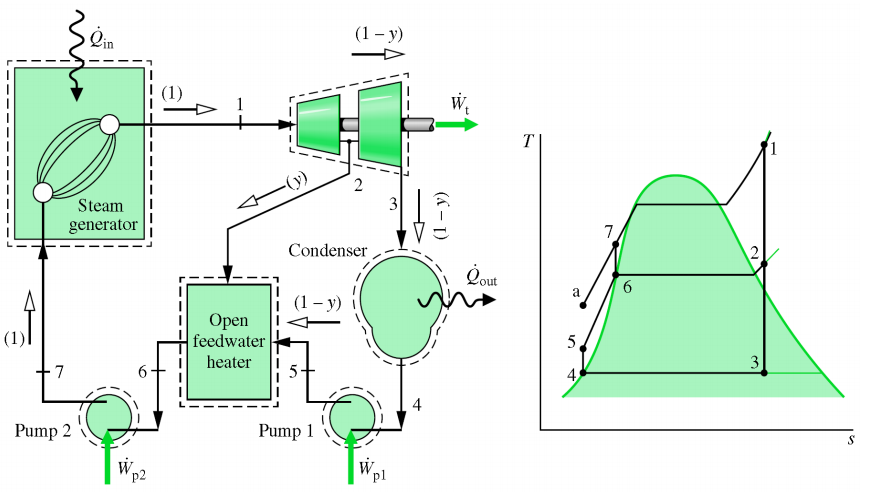
\includegraphics[width = 1 \textwidth]{../img/diagram149.png}
  \caption{Regenerative vapour power cycle with one open feedwater heater}
\end{figure}
\begin{figure}[H]
  \centering
  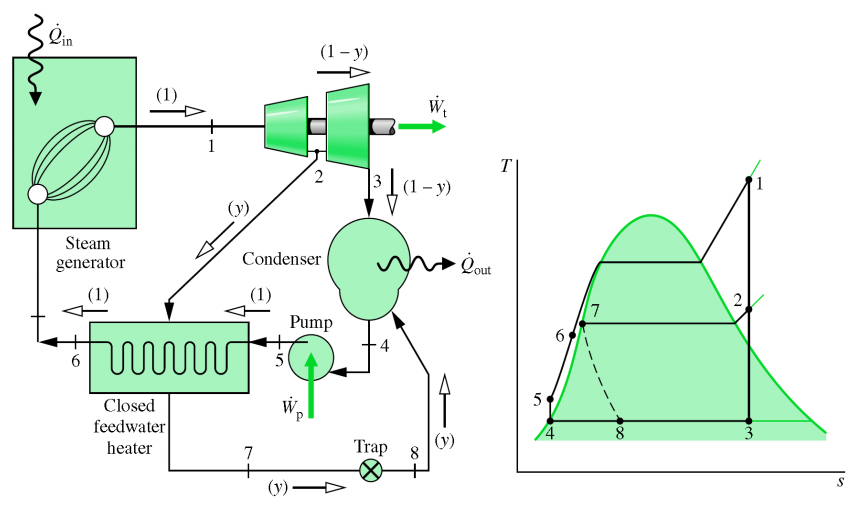
\includegraphics[width = 1 \textwidth]{../img/diagram150.png}
  \caption{Regenerative vapour power cycle with one closed feedwater heater}
\end{figure}
\end{document}